%%%%%%%%%%%%%%%%%%%%%%%%%%%%%%%%%%%%%%%%%
% Beamer Presentation
% LaTeX Template
% Version 1.0 (10/11/12)
%
% This template has been downloaded from:
% http://www.LaTeXTemplates.com
%
% License:
% CC BY-NC-SA 3.0 (http://creativecommons.org/licenses/by-nc-sa/3.0/)
%
%%%%%%%%%%%%%%%%%%%%%%%%%%%%%%%%%%%%%%%%%

%----------------------------------------------------------------------------------------
%	PACKAGES AND THEMES
%----------------------------------------------------------------------------------------

\documentclass{beamer}

\mode<presentation> {

% The Beamer class comes with a number of default slide themes
% which change the colors and layouts of slides. Below this is a list
% of all the themes, uncomment each in turn to see what they look like.

%\usetheme{default}
%\usetheme{AnnArbor}
%\usetheme{Antibes}
%\usetheme{Bergen}
%\usetheme{Berkeley}
%\usetheme{Berlin}
%\usetheme{Boadilla}
%\usetheme{CambridgeUS}
%\usetheme{Copenhagen}
%\usetheme{Darmstadt}
%\usetheme{Dresden}
%\usetheme{Frankfurt}
%\usetheme{Goettingen}
%\usetheme{Hannover}
%\usetheme{Ilmenau}
%\usetheme{JuanLesPins}
%\usetheme{Luebeck}
\usetheme{Madrid}
%\usetheme{Malmoe}
%\usetheme{Marburg}
%\usetheme{Montpellier}
%\usetheme{PaloAlto}
%\usetheme{Pittsburgh}
%\usetheme{Rochester}
%\usetheme{Singapore}
%\usetheme{Szeged}
%\usetheme{Warsaw}

% As well as themes, the Beamer class has a number of color themes
% for any slide theme. Uncomment each of these in turn to see how it
% changes the colors of your current slide theme.

%\usecolortheme{albatross}
%\usecolortheme{beaver}
%\usecolortheme{beetle}
%\usecolortheme{crane}
%\usecolortheme{dolphin}
%\usecolortheme{dove}
%\usecolortheme{fly}
%\usecolortheme{lily}
%\usecolortheme{orchid}
%\usecolortheme{rose}
%\usecolortheme{seagull}
%\usecolortheme{seahorse}
%\usecolortheme{whale}
%\usecolortheme{wolverine}

%\setbeamertemplate{footline} % To remove the footer line in all slides uncomment this line
%\setbeamertemplate{footline}[page number] % To replace the footer line in all slides with a simple slide count uncomment this line

%\setbeamertemplate{navigation symbols}{} % To remove the navigation symbols from the bottom of all slides uncomment this line
}

\usepackage{graphicx} % Allows including images
\usepackage{booktabs} % Allows the use of \toprule, \midrule and \bottomrule in tables
\usepackage{listings}
\usepackage{amsmath}
\usepackage{algpseudocode,algorithm,algorithmicx}

\lstdefinestyle{customjava}{
  breaklines=true,
  frame=L,
  xleftmargin=\parindent,
  language=Java,
  showstringspaces=false,
  basicstyle=\footnotesize\ttfamily,
  keywordstyle=\bfseries\color{green!40!black},
  commentstyle=\itshape\color{gray!40!black},
  identifierstyle=\color{blue},
  stringstyle=\color{orange},
}

\lstdefinestyle{customcpp}{
  breaklines=true,
  frame=L,
  xleftmargin=\parindent,
  language=C++,
  showstringspaces=false,
  basicstyle=\footnotesize\ttfamily,
  keywordstyle=\bfseries\color{green!40!black},
  commentstyle=\itshape\color{gray!40!black},
  identifierstyle=\color{blue},
  stringstyle=\color{orange},
}
%----------------------------------------------------------------------------------------
%	TITLE PAGE
%----------------------------------------------------------------------------------------

\title[Single Cycle]{Single Cycle} % The short title appears at the bottom of every slide, the full title is only on the title page

\author{Jonathan Windle} % Your name
\institute[UEA] % Your institution as it will appear on the bottom of every slide, may be shorthand to save space
{
University of East Anglia \\ % Your institution for the title page
\medskip
\textit{J.Windle@uea.ac.uk} % Your email address
}
\date{\today} % Date, can be changed to a custom date

\begin{document}

\begin{frame}
\titlepage % Print the title page as the first slide
\end{frame}

\begin{frame}[allowframebreaks]
\frametitle{Overview} % Table of contents slide, comment this block out to remove it
\tableofcontents % Throughout your presentation, if you choose to use \section{} and \subsection{} commands, these will automatically be printed on this slide as an overview of your presentation
\end{frame}

%-------------------------------------------------------------------
\section{State Machines}
\begin{frame}
\frametitle{State Machines}
\begin{itemize}
\item Computers are state machines
\item Built from combinational and state elements
\item Combinational element outputs depend only on their inputs
\begin{itemize}
\item e.g. gates, ALU
\end{itemize}
\item State elements hole state i.e. have some internal storage
\begin{itemize}
\item E.g. registers, instruction and data memories
\item {\color{red}Clocking methodology} defines when data can be read and written
\item We will assume {\color{green}positive edge-triggered} clocking.
\end{itemize}
\item Edge-triggered clocking methodology allows for reading a state element and writing in the same clock cycle
\item The clock needs to be long enough so that the input to the state element is stable before the positive clock edge starts.
\end{itemize}
\end{frame}
%------------------------------------------------------------------
\section{Instruction and Data Memories}
\begin{frame}
\frametitle{Instruction and Data Memories}
\begin{itemize}
\item All buses are 32 bits
\item Blue connectors represent control signals. {\color{blue}MemWrite} or {\color{blue}MemRead} should be {\color{red}asserted} (logical high) depending whether we want to write or read from memory
\item For simplicity, assume cannot write to instruction memory - program already there.
\end{itemize}
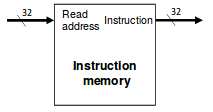
\includegraphics[scale=0.4]{instr.png}
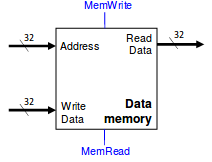
\includegraphics[scale=0.4]{dmem.png}
\end{frame}
%------------------------------------------------------------------
\section{Instruction Fetch}
\begin{frame}
\frametitle{Instruction Fetch}
\begin{itemize}
\item The CPU fetches instructions from the instruction memory and executes them
\item The program counter PC stores the address of the current instruction
\item We also need an adder to increase PC
\begin{itemize}
\item MIPS instructions are one word long, so the PC should be incremented by four to read the subsequent instruction
\end{itemize}
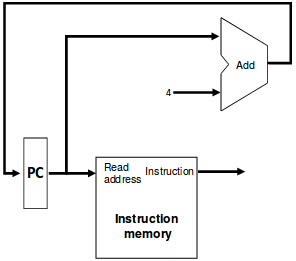
\includegraphics[scale=0.4]{infetch.png}
\end{itemize}
\end{frame}
%--------------------------------------------------------------------
\section{R-type recap}
\begin{frame}
\frametitle{R-type recap}
\begin{itemize}
\item Arithmetic instructions use R-format
\item Three-register-addresss instructions for data manipulations:
\begin{itemize}
\item R:rd$\leftarrow$ funct rt
\end{itemize}
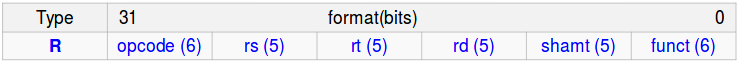
\includegraphics[scale=0.4]{r.png}
\end{itemize}
\end{frame}
%-----------------------------------------------------------------
\section{Register File and ALU}
\begin{frame}
\frametitle{Register File and ALU}
\begin{itemize}
\item R-type instructions require registers and ALU
\item There are 32 registers in the MIPS register file.
\item We need 5 bits to address registers
\item We have 5 operations to encode so ALUop needs to have 3 bits
\end{itemize}
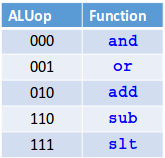
\includegraphics[scale=0.35]{alufunc.png}
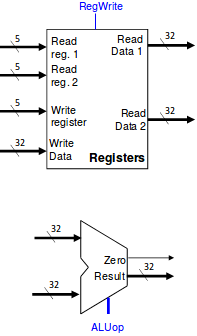
\includegraphics[scale=0.4]{regALU.png}
\end{frame}
%-------------------------------------------------------------------
\section{Executing R-type Instructions}
\begin{frame}
\frametitle{Executing R-type Intructions}
\begin{itemize}
\item Instruction is fetched from memory
\item {\color{red}rs} and {\color{red}rt} registers are read from the register file
\item The ALU operates on the data read. ALU function determined by the {\color{blue}funct} field - bits [0:5] of the instruction
\item The result is written into the {\color{red}rd}
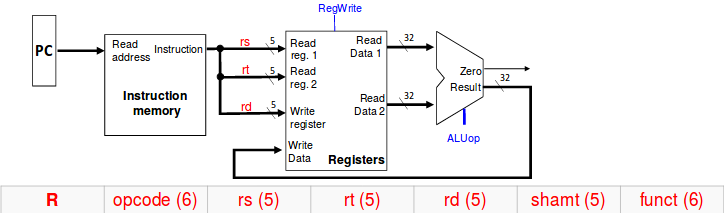
\includegraphics[scale=0.4]{rexec.png}
\end{itemize}
\end{frame}
%------------------------------------------------------------------
\section{I-Type Instruction Recap}
\begin{frame}
\frametitle{I-Type Instruction Recap}
\begin{itemize}
\item I-type instructions include {\color{blue}lw,sw} and {\color{blue}beq}
\item {\color{red}rt} is the destination for {\color{blue}lw} but a source for both {\color{blue}sw \& beq}
\begin{itemize}
\item {\color{blue}lw \$rt, imm(\$rs)}
\item {\color{blue}sw \$rt, imm(\$rs)}
\item {\color{blue}beq \$rs, \$rt, imm}
\end{itemize}
\item {\color{red}immediate} is a 16-bit signed constant (two's complement)
\end{itemize}
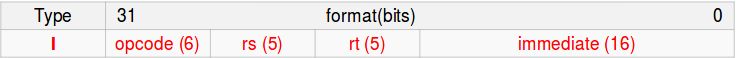
\includegraphics[scale=0.4]{itype.png}
\end{frame}
%------------------------------------------------------------------
\section{Executing Load/Store Instructions}
\begin{frame}
\frametitle{Executing Load/Store Instructions}
\begin{itemize}
\item For load/store instructions, the base register {\color{red}rs} is added to the {\color{red}sign-extended} immediate operand producing a data memory address
\item The ALU must accept either a register operand for arithmetic instructions or a sign-extended immediate operand for load/store instructions
\item We had to add additional three {\color{red}multiplexors} with their control signals.
\end{itemize}
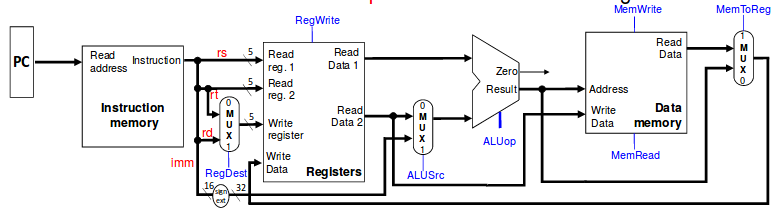
\includegraphics[scale=0.35]{loadstore.png}
\end{frame}
%------------------------------------------------------------------
\section{ALUSrc Control Signal}
\begin{frame}
\frametitle{ALUSrc Control Signal}
\begin{itemize}
\item When asserted selects an {\color{red} immediate} operand, otherwise a {\color{green}register} operand.
\end{itemize}
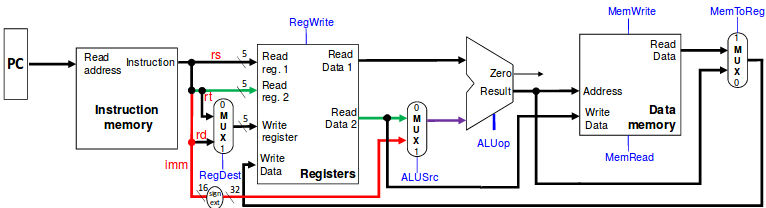
\includegraphics[scale=0.4]{alusrc.png}
\end{frame}
%------------------------------------------------------------------
\section{MemToReg Control Signal}
\begin{frame}
\frametitle{MemToReg Control Signal}
\begin{itemize}
\item When asserted selects storing the data {\color{red}data memory contents} in a register, otherwise it stores the {\color{green}result of the ALU operation}
\end{itemize}
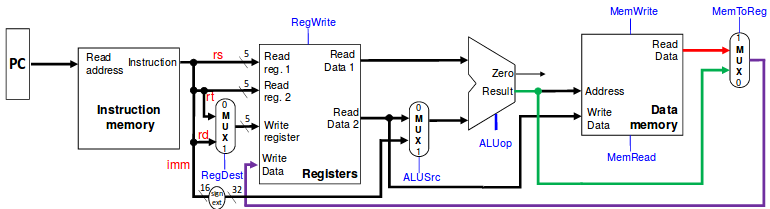
\includegraphics[scale=0.4]{memreg.png}
\end{frame}
%-------------------------------------------------------------------
\section{RegDest Control Signal}
\begin{frame}
\frametitle{RegDest Control Signal}
\begin{itemize}
\item We need one more mux for selecting the destination register, which is different in R and I-type instructions
\item When asserted selects storing the result in a register {\color{red}rd(R-type)} otherwise it stores the result in the {\color{green}rt} register {\color{green}(lw,I-type)}.
\end{itemize}
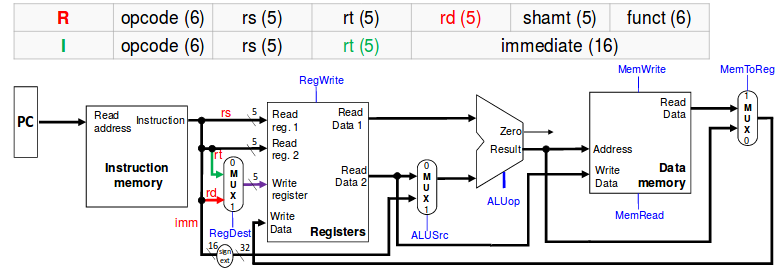
\includegraphics[scale=0.4]{regdest.png}
\end{frame}
%-----------------------------------------------------------------
\section{Branch Instruction Recap}
\begin{frame}
\frametitle{Branch Instruction Recap}
\begin{itemize}
\item In branch instructions the immediate operand is not an address offset, but the instruction offset:
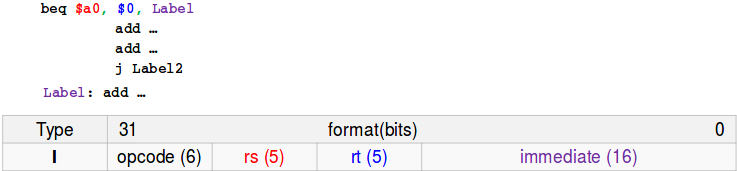
\includegraphics[scale=0.4]{brec.png}
\item {\color{purple}Label} is three instructions after the instruction immediately following beq, hence the offset will be three words (twelve bytes) i.e. the branch address equals PC+4+imm$\times$4
\item Of course, the offset is a signed integer (two's complement)
\end{itemize}
\end{frame}
%------------------------------------------------------------------

\begin{frame} 
\Huge{\centerline{The End}}
\end{frame}

\end{document}